\section{Results}
\label{sec:results}

\subsection{Site and wind}

The abbey stands \SI{\nRelief}{\meter} above the valley floor on a spur whose flanks face
southwest (aspect \ang{\nAspect}), with a mean slope of \ang{\nSlopeMean} and a
90th-percentile slope of \ang{\nSlopePninety} within \SI{\nSlopeRadius}{\meter}
(\cref{fig:site}).
The southwest-facing ground near the abbey forms a strip \SI{\nLiftAlongSlope}{\meter} long
running northwest from the abbey; heading southwest, the ground reaches the valley floor
within \SI{\nLiftIntoWind}{\meter}.

Over twenty years the wind blows from the southwest sector at
\SIrange{5}{12}{\meter\per\second} in \SI{\nFavPct}{\percent} of hours
(\SI{95}{\percent} CI \SIrange{\nFavLo}{\nFavHi}{\percent}), about \nFavHours\ hours a year,
and in \SI{\nFavWinter}{\percent} of winter hours (\cref{fig:wind}).
Strong southwest winds are rarer: \SI{6}{\meter\per\second} or more in
\SI{\nSWSixPct}{\percent} of hours (\nSWSixHours\ hours a year), and
\SI{8}{\meter\per\second} or more in \SI{\nSWEightPct}{\percent}
(CI \SIrange{\nSWEightLo}{\nSWEightHi}{\percent}; \nSWEightHours\ hours a year).

\begin{figure}[htbp]
  \centering
  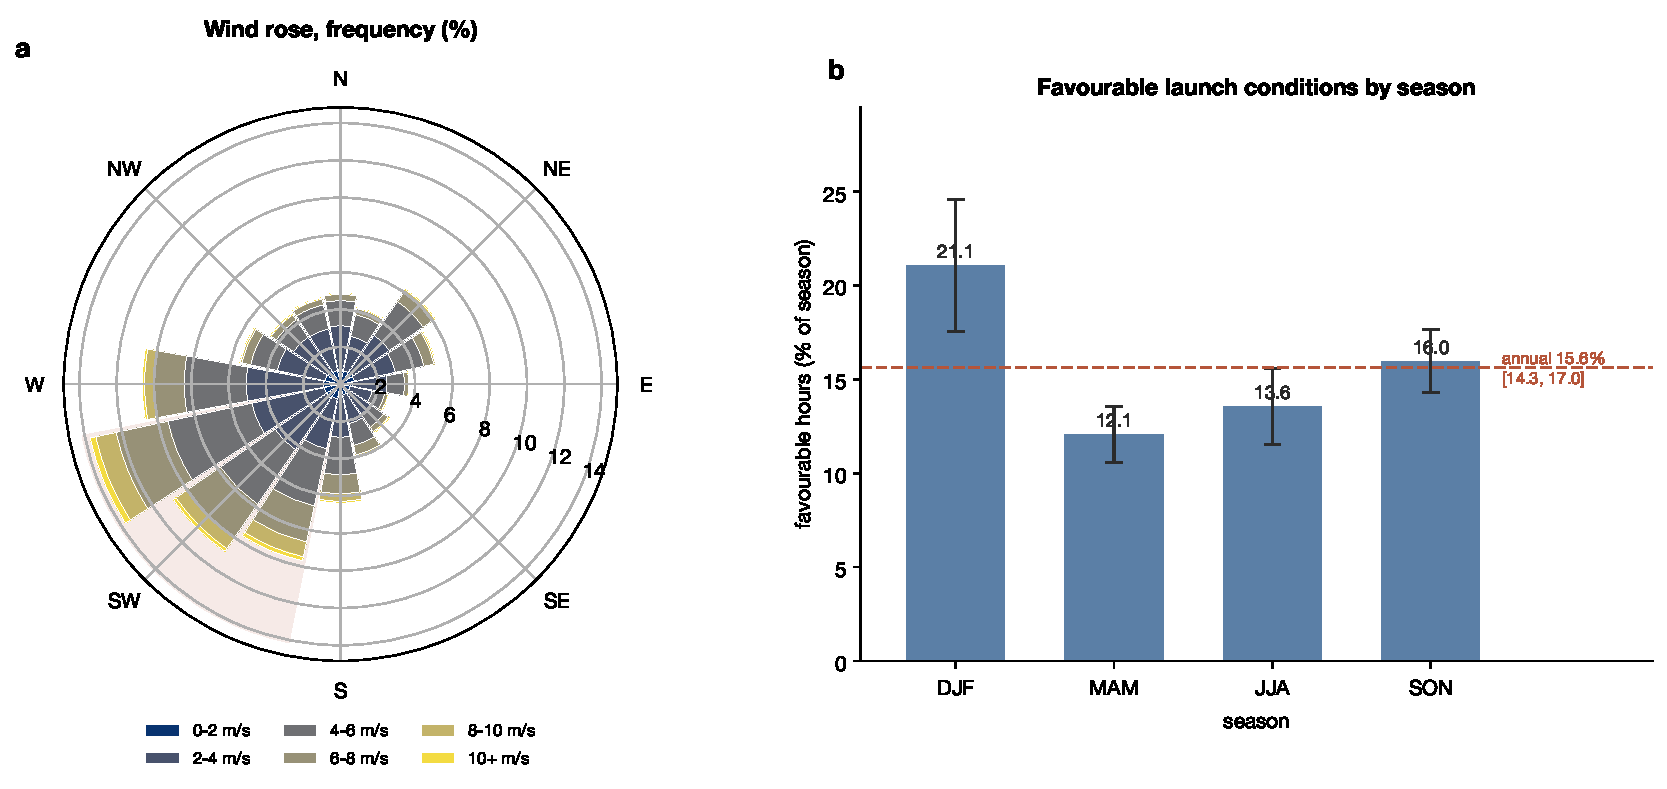
\includegraphics[width=\linewidth]{fig2_wind}
  \caption{\textbf{Wind at the abbey, 2004--2023.}
  \textbf{(a)} Wind rose of ERA5 hourly \SI{10}{\meter} wind (\nHours\ hours).
  \textbf{(b)} Fraction of hours from the southwest sector (\ang{191}--\ang{259}) at
  \SIrange{5}{12}{\meter\per\second}, for the year and by season (DJF, December--February;
  MAM, March--May; JJA, June--August; SON, September--November), with \SI{95}{\percent}
  confidence intervals across the twenty years.}
  \label{fig:wind}
\end{figure}

The linear model (\cref{eq:ridge}) gives a peak upward air speed of
\SI{\nRidgePeak}{\meter\per\second} just southwest of the abbey in an
\SI{\nRidgeWind}{\meter\per\second} wind (Supplementary \cref{fig:ridge}), close to the
surface estimate \(U\sin\theta_s = \SI{\nRidgeFormula}{\meter\per\second}\) at the
90th-percentile slope.
The still-air sink rate of the nominal craft at its best glide is
\(V/\sqrt{1+(\LD)^2}\): \SI{\nSinkBest}{\meter\per\second} at \LD~\num{\nLDhi} and
\SI{\nSinkNominal}{\meter\per\second} at \LD~\num{\nLDnom}.
Ridge lift can therefore roughly cancel the sink of the better wings in a strong wind, and
not that of the poorer ones.

\subsection{Launch and glide}

In still air, a steady glide from the \SI{\nTower}{\meter} tower would cover
\SI{200}{\meter} only with \LD~\num{\nLDStillSteady}, beyond the range of
\cref{eq:polar}.
A standing launch does much worse.
Reaching \SI{\nTrimSpeed}{\meter\per\second} from \SI{\nJump}{\meter\per\second} costs
\((V^2 - v_0^2)/2g \approx \SI{\nHeightToTrim}{\meter}\) of height, and the best wing,
\LD~\num{\nLDhi}, lands \SI{\nStillRangeBest}{\meter} from the tower instead of the
\SI{\nStillRangeSteady}{\meter} of a steady glide (\cref{fig:glide}b).
A headwind supplies airspeed at release without the dive, which is why the wind matters for
the launch as well as for the lift.

Into the wind, the headwind that eases the launch also slows the craft over the ground,
and the lift ends within \SI{\nLiftIntoWind}{\meter}.
None of the three wings in \cref{fig:glide}a reaches \SI{200}{\meter} on this track at any
wind up to \SI{14}{\meter\per\second}; the longest flight is \SI{\nMaxRangeInto}{\meter}
(dashed lines).
Along the slope, the lift lasts for \SI{\nLiftAlongSlope}{\meter}, and a crabbing craft can
stay in it.
The best wing reaches \SI{200}{\meter} from a \SI{\nTower}{\meter} tower above
\SI{\nMinWindBest}{\meter\per\second} of wind and the central wing above
\SI{\nMinWindNominal}{\meter\per\second}; the poorest wing does not reach it at any wind
(\cref{fig:glide}a, solid).
The threshold for the best wing moves from \SI{\nMinWindTowerHi}{\meter\per\second} to
\SI{\nMinWindTowerLo}{\meter\per\second} as the tower height falls from \SI{25}{\meter} to
\SI{15}{\meter}.

\begin{figure}[htbp]
  \centering
  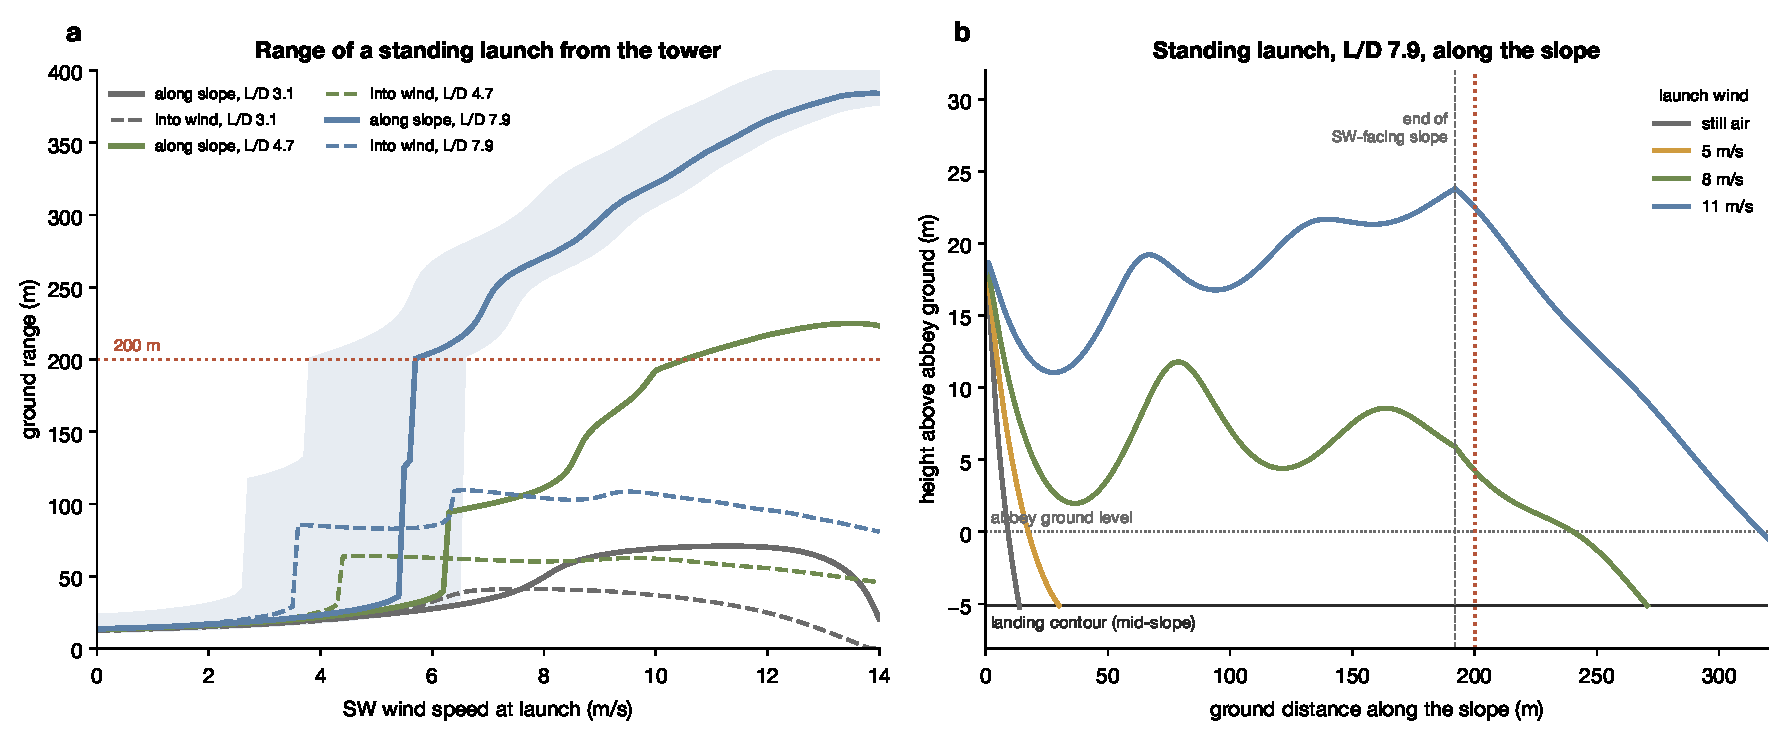
\includegraphics[width=\linewidth]{fig4_glide_envelope}
  \caption{\textbf{Range of a standing launch from the tower.}
  \textbf{(a)} Ground range against launch wind for the nominal craft (\cref{fig:apparatus})
  launched from \SI{\nTower}{\meter} at \SI{\nJump}{\meter\per\second}, for the lowest,
  central, and highest glide ratios of the drag-polar range, on the track along the slope
  (solid) and into the wind (dashed).
  The shaded band is the best wing along the slope for towers of \SIrange{15}{25}{\meter}.
  The step near \SI{5.5}{\meter\per\second} is where ridge lift first matches the sink of
  the best wing.
  \textbf{(b)} Trajectories along the slope for the best wing (\LD~\num{\nLDhi}).
  In still air the craft dives to gain speed and lands \SI{\nStillRangeBest}{\meter} out; in
  wind it climbs and falls in the lift and descends once past the end of the
  southwest-facing slope.}
  \label{fig:glide}
\end{figure}

\subsection{Pitch stability}

Without a tail the neutral point is at \num{\nNPnotail}\,\(c\), ahead of every sampled CG,
so the wing is statically unstable in pitch (\cref{fig:stability}).
Pitch damping delays the divergence until the CG is aft of \num{\nCGonset}\,\(c\).
Across the sampled CG range the doubling time falls from \SI{\nTdoubleFwd}{\second} at
\num{\nCGlo}\,\(c\) to \SI{\nTdoubleAft}{\second} at \num{\nCGhi}\,\(c\)
(\SIrange{\nTdoubleInLo}{\nTdoubleInHi}{\second} when the pitch inertia is halved or
doubled); a \SI{200}{\meter} flight of the nominal craft lasts about
\SI{\nFlightTime}{\second}.
After an \ang{8} gust the tailless craft passes \ang{60} of pitch in
\SI{\nTloss}{\second}.
With a tail the same gust dies away.

\begin{figure}[htbp]
  \centering
  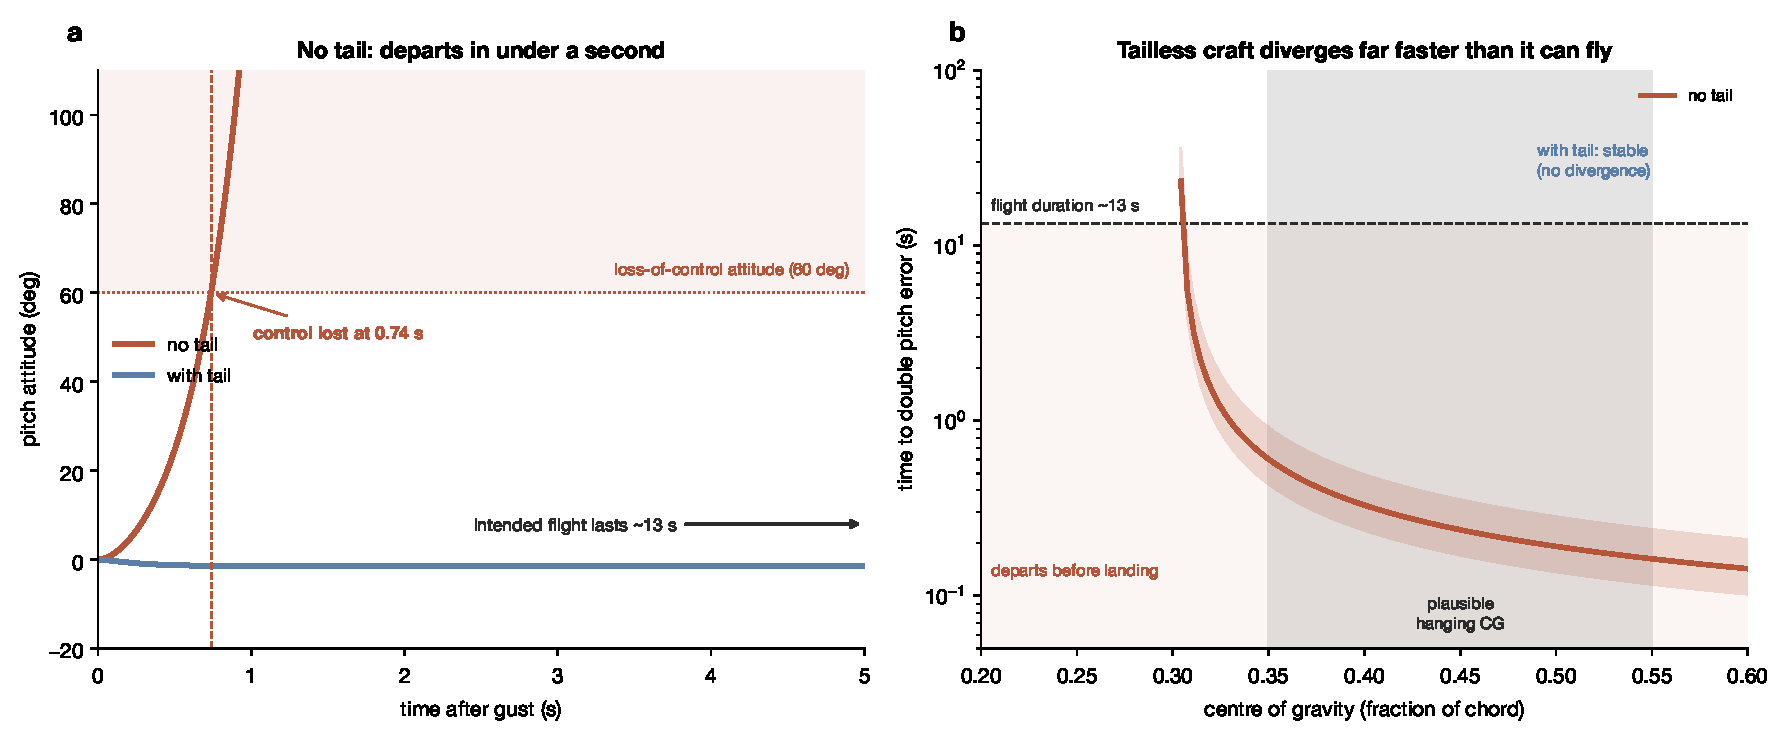
\includegraphics[width=\linewidth]{fig5_stability}
  \caption{\textbf{Pitch stability with and without a tail.}
  \textbf{(a)} Pitch attitude after an \ang{8} gust for the nominal craft with its CG at
  mid-range.
  Without a tail the attitude passes \ang{60} after \SI{\nTloss}{\second}; with a tail the
  disturbance damps out.
  \textbf{(b)} Time for a pitch disturbance to double against CG position for the tailless
  craft; the band is pitch inertia from half to twice nominal.
  The grey band is the sampled CG range and the tan band the effective time delay of a human
  operator \autocite{mcruer1967pilot}.
  The tailed craft does not diverge at any CG shown.}
  \label{fig:stability}
\end{figure}

\subsection{Monte Carlo sample}

Into the wind, none of the \nSamples\ cases reaches \SI{200}{\meter}
(\SI{95}{\percent} upper bound \SI{\nReachIntoHi}{\percent}); the median range is
\SI{\nMedRangeInto}{\meter} (\cref{fig:montecarlo}a).
Along the slope, \nReachSlopeN\ cases do, \SI{\nReachSlope}{\percent}
(CI \SIrange{\nReachSlopeLo}{\nReachSlopeHi}{\percent}), against a median range of
\SI{\nMedRangeSlope}{\meter} and a 90th percentile of \SI{\nNinetyRangeSlope}{\meter}.
The cases that reach it share a strong wind and a good wing: their median launch wind is
\SI{\nMedWindReach}{\meter\per\second} (\SI{90}{\percent} above
\SI{\nTenWindReach}{\meter\per\second}), and their median glide ratio is \num{\nMedLDReach},
against \num{\nMedLDAll} over all cases.
\SI{\nShortFifty}{\percent} of all cases land within \SI{50}{\meter} of the tower.

Among the cases that reach \SI{200}{\meter}, the tailless doubling time has a median of
\SI{\nTdoubleMC}{\second} (99th percentile \SI{\nTdoubleMCpnn}{\second}) and the flight a
median of \SI{\nMedFlightReach}{\second} (\cref{fig:montecarlo}b).
In every one of them the doubling time is shorter than the flight, and with a tail none
diverges.

\begin{figure}[htbp]
  \centering
  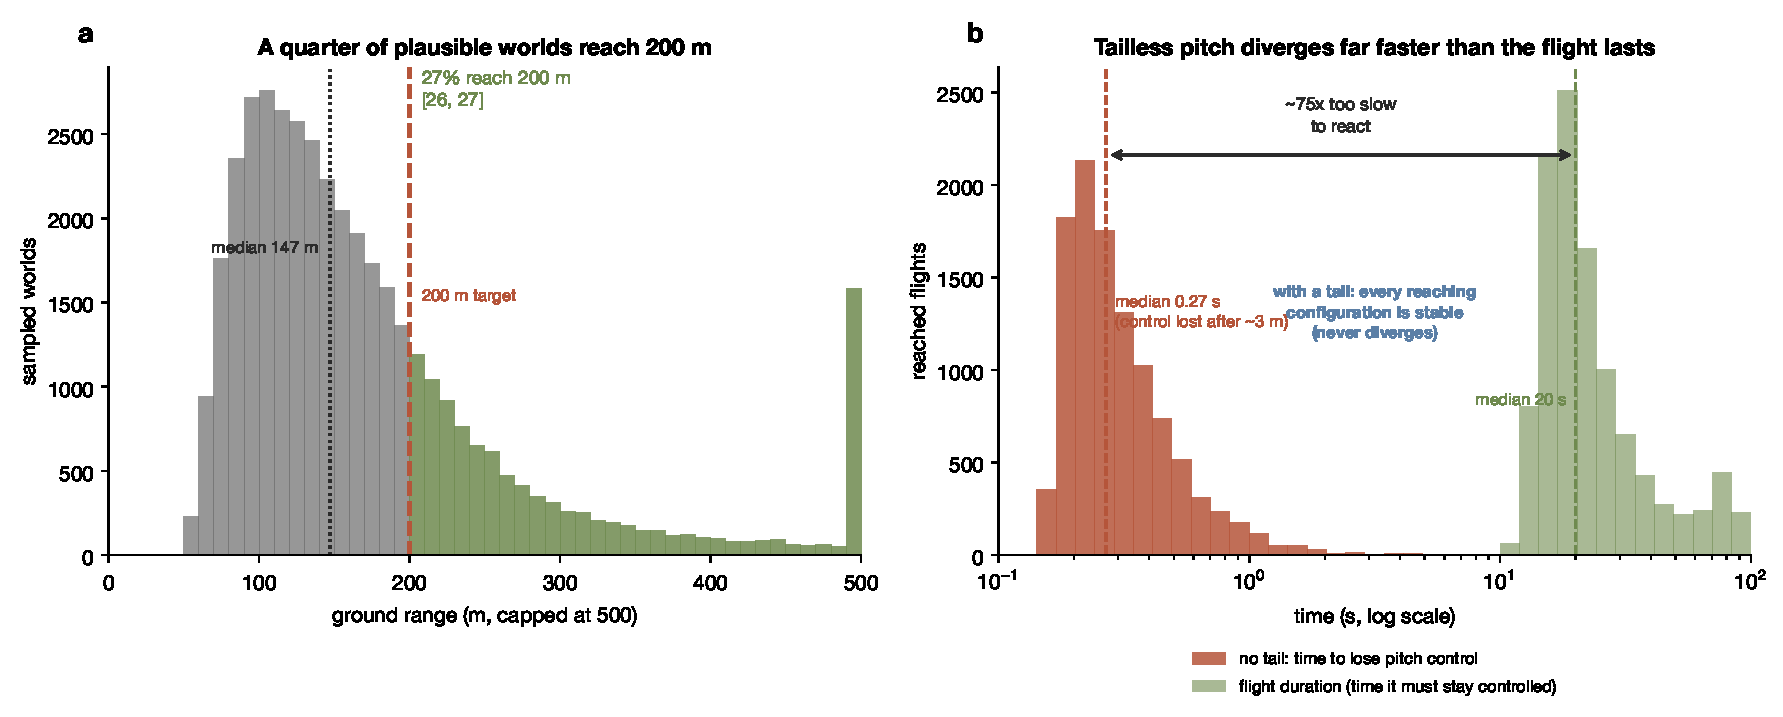
\includegraphics[width=\linewidth]{fig6_montecarlo}
  \caption{\textbf{Monte Carlo sample of \nSamples\ apparatus and launch-day cases.}
  Parameters are drawn from Supplementary \cref{tab:priors}, and the launch wind from the
  ERA5 southwest-sector hours.
  \textbf{(a)} Ground range on the two tracks.
  Along the slope \SI{\nReachSlope}{\percent} of cases reach \SI{200}{\meter}
  (\SI{95}{\percent} CI \SIrange{\nReachSlopeLo}{\nReachSlopeHi}{\percent}); into the wind
  none does.
  \textbf{(b)} For the \nReachSlopeN\ cases that reach \SI{200}{\meter} along the slope, the
  time for a pitch disturbance to double without a tail, and the duration of the flight.
  The tan band is the effective time delay of a human operator.}
  \label{fig:montecarlo}
\end{figure}

\subsection{Impact}

For \(d = \SI{20}{\centi\meter}\) the legs break above about
\SI{\nOnsetMid}{\meter\per\second} of vertical speed, and the onset ranges from
\SI{\nOnsetLo}{\meter\per\second} to \SI{\nOnsetHi}{\meter\per\second} across the stopping
distances and fracture loads (\cref{fig:biomech}a).
A controlled glide that ends without a flare meets the ground at a median
\SI{\nCtrlVzMed}{\meter\per\second} and at most \SI{\nCtrlVzMax}{\meter\per\second} of
vertical speed, below the lowest onset speed, so it does not break the legs even without a
flare (\cref{fig:biomech}b).
An arrival after loss of pitch control, at airspeeds of
\SIrange{\nVreachLo}{\nVreachHi}{\meter\per\second}, has a median vertical speed of
\SI{\nDepVzMed}{\meter\per\second}; \SI{\nPbreakDep}{\percent} of such arrivals exceed the
central onset speed.
The median deceleration over \SI{20}{\centi\meter} is about \num{\nDecelG}\,\(g\), which
feet-first falls are commonly survived.

\begin{figure}[htbp]
  \centering
  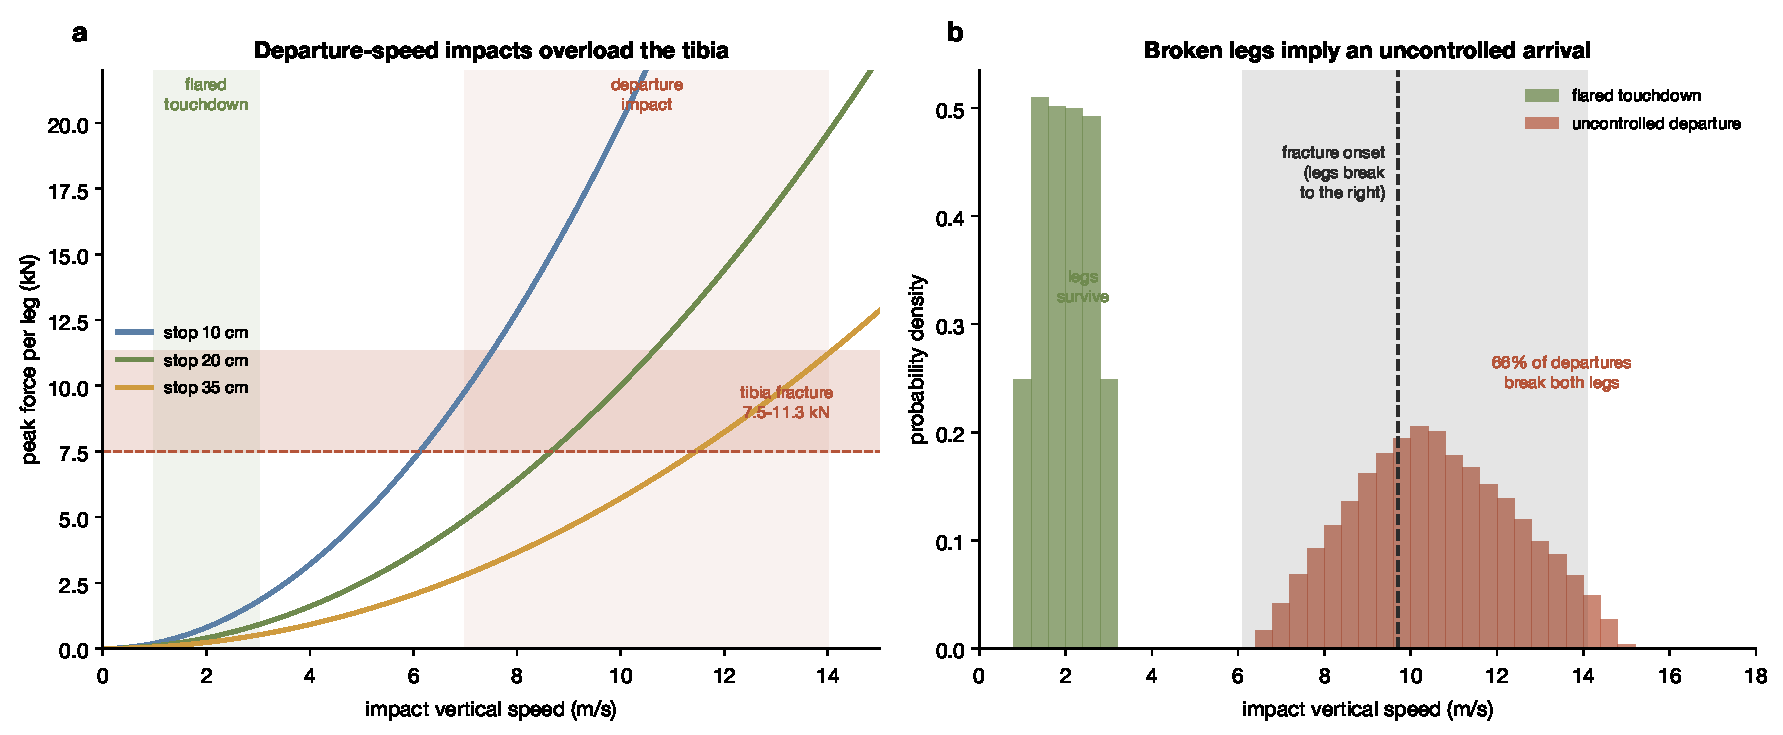
\includegraphics[width=\linewidth]{fig7_biomech}
  \caption{\textbf{Arrival speed and leg fracture.}
  \textbf{(a)} Mean feet-first impact force per leg against vertical speed for stopping
  distances of \SIrange{10}{35}{\centi\meter}, with the tibia fracture range
  (\SIrange{\nTibiaLo}{\nTibiaHi}{\kilo\newton} per leg).
  \textbf{(b)} Vertical arrival speeds of the \nReachSlopeN\ cases that reach
  \SI{200}{\meter}, for a controlled glide that ends without a flare and for an arrival
  after loss of pitch control (\(V\sin\theta\), \(\theta =
  \ang{\nDepAngLo}\text{--}\ang{\nDepAngHi}\)).
  The grey band is the range of fracture-onset speeds and the dashed line its centre.}
  \label{fig:biomech}
\end{figure}
\FloatBarrier
